%% This is an example first chapter.  You should put chapter/appendix that you
%% write into a separate file, and add a line \include{yourfilename} to
%% main.tex, where `yourfilename.tex' is the name of the chapter/appendix file.
%% You can process specific files by typing their names in at the 
%% \files=
%% prompt when you run the file main.tex through LaTeX.
\chapter{Generating Control-Flow-Enriched Data Flows from User Programs}
This chapter revolves around intermediate code generation part of the compiler in which translation of the source program into target code takes place. In the process of translating a program written in a given language into code for a given target machine, a compiler typically constructs a sequence of intermediate representation which can have a variety of forms \cite{lam2006compilers}. High-level representations are close to the source language and low-level representations are close to the target machine. Syntax tree is one of the most commonly used forms of high-level intermediate representation during syntax and semantic analysis. During intermediate code generation phase of the compiler, another set of intermediate representation i.e. control flow graph is produced. In the preliminaries section of this chapter, we present overview of the theory around syntax trees and graph in order to equip the reader with necessary knowledge to understand how to generate the control-flow enriched data flows from given user programs which we talk about later in this chapter. 

\section{Preliminaries}
\subsection{Syntax Directed Translation}
Before going through the intermediate code generation phase of the compiler, we first visit its preliminary phase which is the Syntax-Directed Translation phase in which the translation of languages guided by context-free grammars is developed (for formal explanation of context-free grammars, refer to Definition \ref{def:grammar}). The parser uses the components produced by the lexical analyzer to create a tree-like intermediate representation depicting the grammatical structure of the source program \cite{lam2006compilers}. This translation technique will be applied in intermediate code generation. The most general approach to syntax-directed translation is to construct a syntax tree and to compute the values of attributes at the node of the tree by visiting all the nodes \cite{lam2006compilers}. Information is associated with the syntax tree by attaching attributes to the grammar symbols representing the programming construct.

Syntax-Directed Definition (SDD) is context-free grammar completed with attributes and rules. Attributes are associated with grammar symbols and rules are associated with productions. An attribute is any quantity associated with a programming construct. Example of attributes are data types of expressions, the number of instructions in the generated code, or the location of the first instructions in the generated code for a construct. Since we are using grammar symbols (nonterminals and terminals), the notion of attributes is extended from constructs to the symbols that represent them.

A context-free grammar in itself specifies a set of terminal symbols (inputs), another set of nonterminals (e.g. symbols representing syntactic context), and a set of productions. Each of these gives way in which strings represented by one nonterminal can be constructed from terminal symbols and strings represented by other nonterminals. Production consists of a head which is the nonterminals to be replaced and a body which is the replacing string of grammar symbols. There are two kinds of attributes for nonterminals, which are Inherited and Synthesized Attributes. The differences between the two are as follows \cite{lam2006compilers}:
\begin{itemize}
\item Synthesized Attributes. A synthesized attribute for a nonterminal A at a parse-tree node N is defined by a semantic rule associated with the production at N.
\item Inherited Attributes. An inherited attribute for a nonterminal B at a parse-tree node N is defined by a semantic rule associated with the production at the parent of N. Note that the production must have B as a symbol in its body.
\end{itemize}

\begin{definition}[Context-Free Grammars]
A context-free grammar has four components as follow \cite{lam2006compilers}:
\begin{enumerate}
\item A set of terminal symbols. The terminals are the elementary symbols of the language defined by the grammar. 
\item A set of nonterminals. Each nonterminal represents a set of strings of terminals. 
\item A set of productions. Each production consists of a nonterminal, called head or left side of the production, a arrow, and a sequence of terminals and/or nonterminals, called the body or right side of the production. 
\item One of the nonterminals is designed as the start symbol. 
\end{enumerate}
\label{def:grammar}
\end{definition}

\subsection{Abstract Syntax Trees}
During syntax-analysis or parsing, the compiler creates syntax-tree nodes to represent significant programming constructs (e.g. operators, classes, control flow etc). This phase takes the list of tokens produced by the lexical analysis and arranges these in a tree-structure that reflects the structure of the program. The purpose of the syntax analysis or parsing phase is to recombine the tokens produced by the lexical analysis as a result of input splitting into a form that reflects the structure of the source program. This form is typically a data structure called the syntax tree or parse tree of the program. As the name indicates, syntax tree is a tree structure \cite{mogensen2009basics}. As the analysis continues, information is added to the node in the form of attributes associated to the node depending on the translation to be performed \cite{lam2006compilers}.

During syntax-directed translation phase in the compiler, a syntax-directed translator is constructed to translate arithmetic expressions into postfix form (see Definition \ref{def:postfix}). Abstract Syntax Tree (AST) is a data structure that is most useful for designing this syntax-directed translator. In an AST for an expression, each interior node represents an operator whereas the children of the node represent the operand of the operator. The difference between AST and the parse tree is that the AST keeps the essence of the structure of the program but omits the irrelevant details \cite{mogensen2009basics}. It corresponds to one or more nodes in the parse tree. In general, any programming construct can be handled by creating an operator for the construct and treating the semantically meaningful components of that construct as operands \cite{lam2006compilers}. The AST represents an expression formed by applying the operator \textbf{op} to the subexpressions represented by $E_{1}$ and $E_{2}$. It can be created for any construct, not limited to expressions. Each construct is represented by a node, with children for the semantically meaningful components of the construct. An operator in the abstract syntax is defined for every statement construct. For constructs that begin with a keyword, the keyword is used for the operator (e.g. operator \textbf{while} for while-statements). 

We define the scope of the language grammar for our thesis as depicted in Figure \ref{fig:grammardef} and explain the syntax tree for a language based on this grammar. Syntax-tree $Expr$ is used to represent all kinds of expressions, and $stmt$ to represent all kinds of statements. Since a block is a grouping of a program, a syntax tree for a program is of type block. When a statement is a block, it has the same syntax tree as the block (hence, $stmt \to block$). The syntax tree for nonterminal block is simply the syntax tree for the sequence of statements in the block. A sequence of statements is represented by using a leaf \textbf{null}. We ignore declarations in our grammar definition since they are not used in the syntax tree. Blocks, with or without declarations, appear to be just another statement construct in intermediate code. Conditionals can be handled by defining two operators \textbf{ifelse} and \textbf{if} for if-statements with and without an else part, respectively. The syntax tree node for a while-statement and a do-while statement has an operator, which we call \textbf{while} and \textbf{dowhile}, respectively and two children - the syntax trees for the $expr$ and the $stmt$. 

\begin{figure}[here]
\begin{algorithmic}
\State $ program \to block$
\State $ block \to '\{' stmts '\}'$
\State $ stmts \to stmts_{1} stmt $
\State $ stmts \to \epsilon$
\State $ stmt \to expr $
\State $ stmt \to \textbf{if} (expr) stmt_{1}$
\State $ stmt \to \textbf{if} (expr) stmt_{1} else stmt_{2} $
\State $ stmt \to \textbf{while} (expr) stmt_{1}$
\State $ stmt \to \textbf{do} (stmt_{1}) expr $
\State $ stmt \to block $
\end{algorithmic}
\caption{Context-Free Grammar}
\label{fig:grammardef}
\end{figure}

\begin{definition}[Postfix Form]
Postfix form for an expression $E$ can be defined as follows:
\begin{enumerate}
\item If $E$ is a variable or constant, then the postfix form for E is E itself. 
\item If $E$ is an expression of the form $E_{1}$ \textbf{op} $E_{2}$, where \textbf{op} is any binary operator, then the postfix form for $E$ is $E_{1}'$ $E_{2}'$ \textbf{op} where $E_{1}'$ and $E_{2}'$ are the postfix forms of $E_{1}$ and $E_{2}$ respectively. 
\item If $E$ is a parenthesized expression of the form ($E_{1}$), then the postfix form for $E$ is the same as the postfix form for $E_{1}$
\end{enumerate}
\label{def:postfix}
\end{definition}

\subsection{Control-Flow Graphs}
The Control-Flow Graph (CFG) is another intermediate representation that is produced during syntax-analysis . Frances E. Allen \cite{allen1970control} defines a CFG as "a directed graph in which the nodes represent basic blocks and the edges represent control flow paths". The CFG serves as framework for static analysis of program control flow. Many code generators partition intermediate representation instructions into basic blocks, which consist of sequences of instructions or statements that are always executed together \cite{lam2006compilers}. Basic blocks are a straight line, single-entry code with no branching except at the end of the sequence. 

\begin{figure}[h!]
\centering
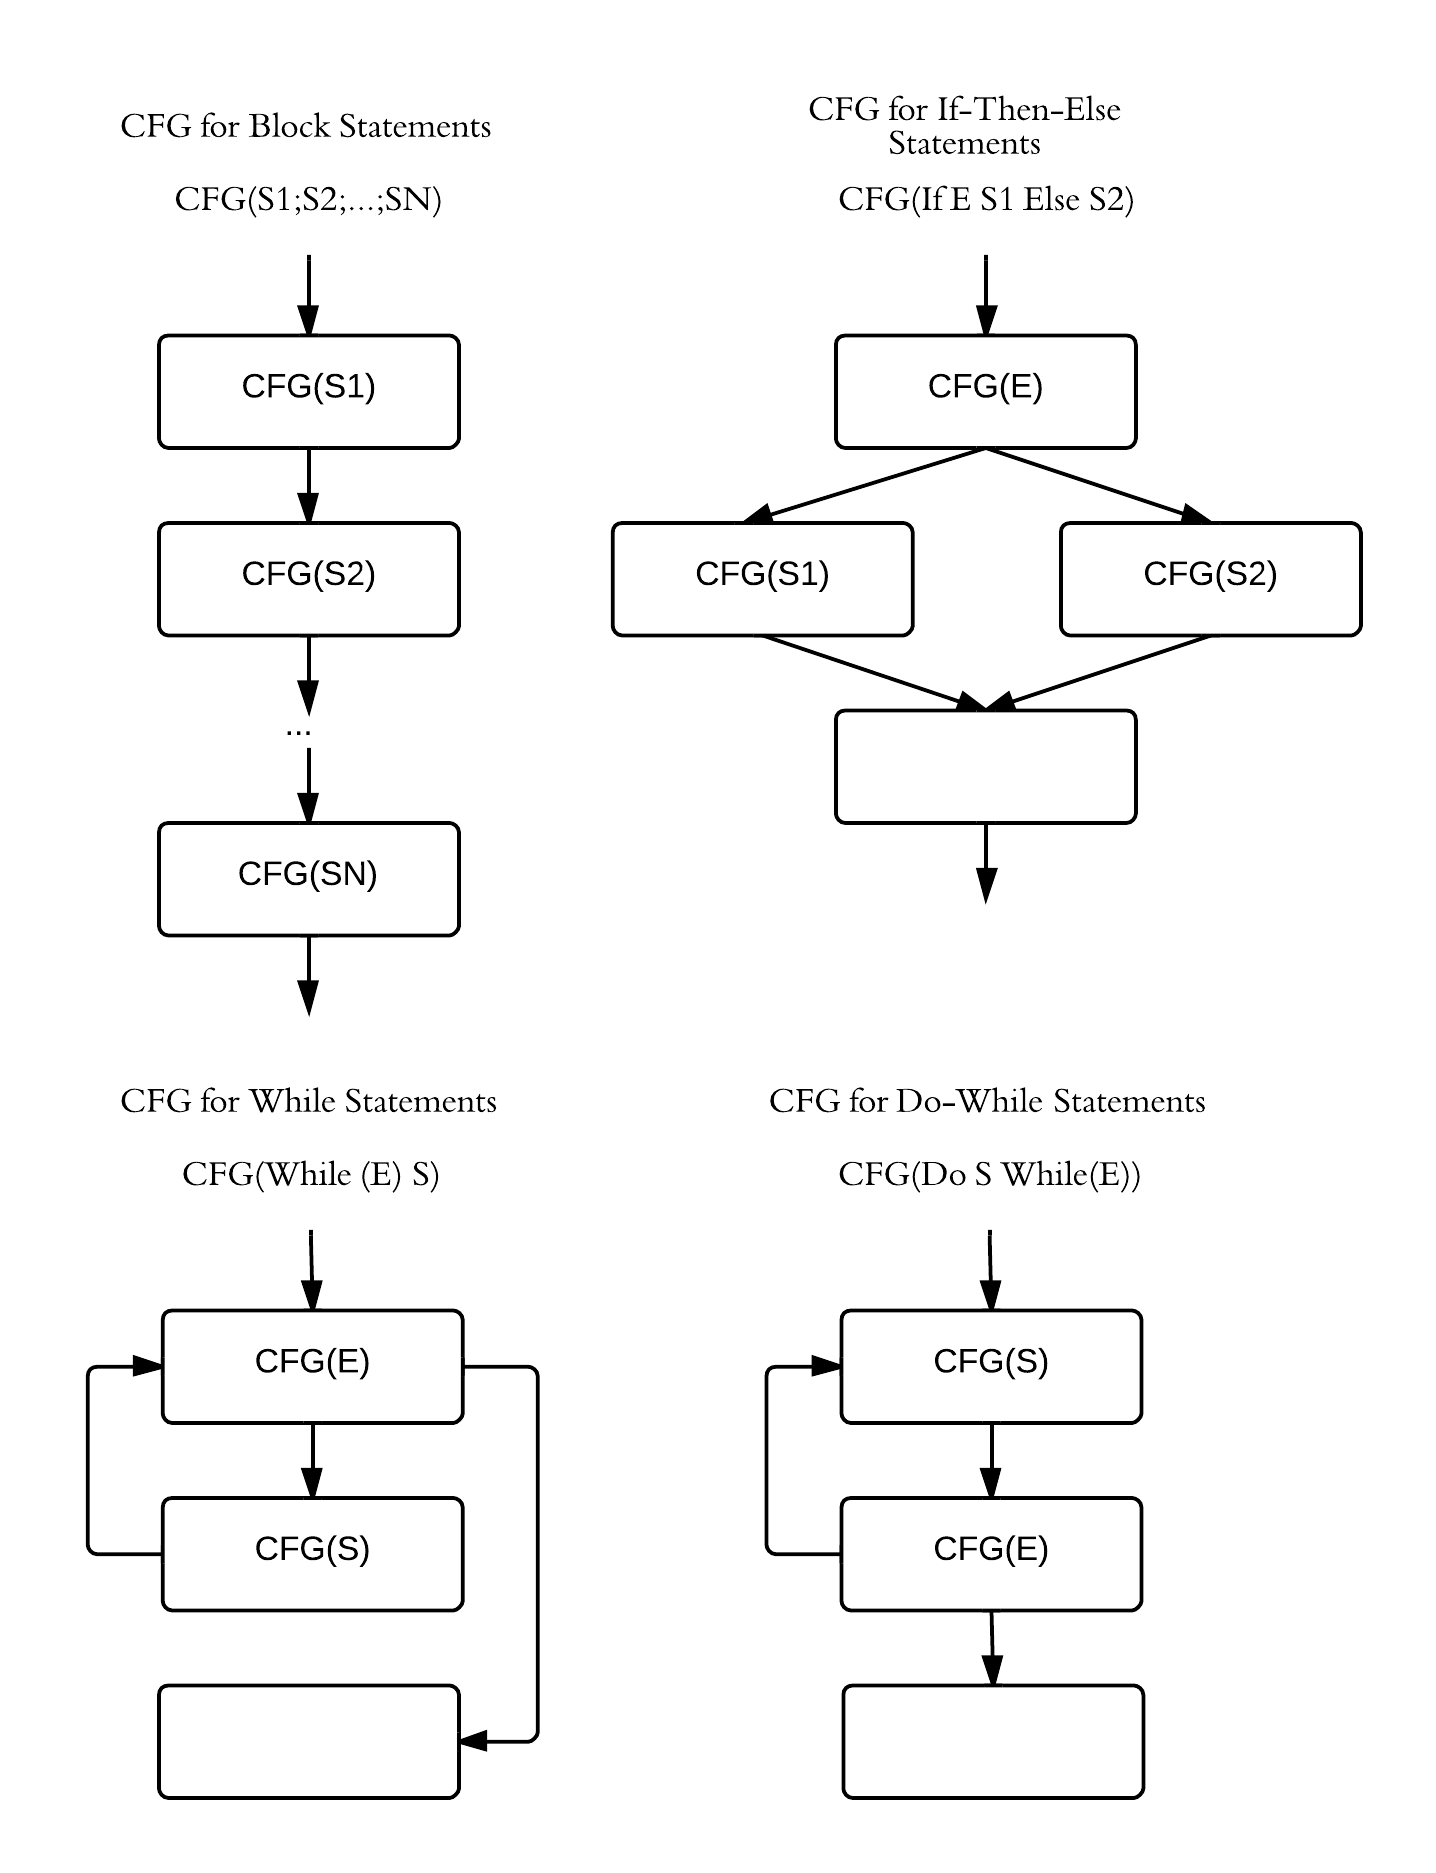
\includegraphics[width=0.7\linewidth]{figures/Graph}
\caption{CFG of Various Statements}
\label{fig:Graph}
\end{figure}

Edges represent possible flow of control from the end of one block to the beginning of the other. There may be multiple incoming or outgoing edges for each block \cite{allen1970control}. After the intermediate code has been partitioned into basic blocks, the flow of control between them can be represented by a CFG. There is an edge from block A to block B if and only if it is possible for the first statement in block B to immediately follow the last statement in block A. Given a Block statement, If-Then-Else statement, and While-statement, we formulate the expected CFG result from the first stage of the algorithm as shown in Figure \ref{fig:Graph}. CFG(S) is a CFG of high-level statement S. CFG(S) is a single entry and single-exit graph with one entry node and one exit node both in the form of a basic block. In the first stage of our algorithm, construction of CFG(S) is recursively defined and will be presented in detailed in the next section. 

\subsection{Data-Flow Analysis}
In the second stage of our algorithm, we analyze the graph to detect data dependencies and subsequently add another type of Edges which show the data dependencies between the nodes of the CFG. Data dependencies describe the normal situation that the data some statements or basic blocks use depends on the data created by other statements or other basic blocks. Data-flow analysis aims to derive information about the flow of data along with program execution paths. In analyzing the behavior of a program, all the possible sequences of program points ("paths") through a CFG that the program execution can take must be considered. From the possible program states at each point, we extract the information we need for the particular data-flow analysis problem to be solved. The possible execution paths in a CFG can be defined as follows \cite{lam2006compilers}.
\begin{itemize}
\item Within one basic block, the program point after a statement is the same as the program point before the next statement. 
\item If there is an edge from block $B_{1}$ to block $B_{2}$, then the program point after the last statement of $B_{1}$ may be followed immediately by the program point before the first statement of $B_{2}$. 
\end{itemize}
In \cite{lam2006compilers}, $Execution\;path$ or $path$ from point $p_{1}$ to point $p_{n}$ is defined as a sequence of points $p_{1}, p_{2}, ..., p_{n}$ such that for each $i = 1, 2, ..., n-1$, either 
\begin{enumerate}
\item $p_{i}$ is the point immediately preceding a statement and $p_{i+1}$ is the point immediately following that same statement, or 
\item $p_{i}$ is the end of some block and $p_{i+1}$ is the beginning of a successor block. 
\end{enumerate}

\subsubsection{Data-Flow Analysis Schema on Basic Blocks}
A \textbf{data-flow value} at a program point represents the set of all possible program states that can be observed for that point, for example, all definitions in the program that can reach that point \cite{lam2006compilers}. We denote the data-flows values immediately before and immediately after each basic block B in a CFG of a program by IN[B] and OUT[B], respectively. A transfer function $f_{B}$ relates the data-flow values before and after a block B. Transfer functions can be either the information that propagate forward along the execution paths, or the information that flow backwards up the execution paths. The \textbf{data-flow problem} for a CFG is to compute the values of IN[B] and OUT[B] for all blocks B in the CFG \cite{lam2006compilers}. 

Suppose block B contains of statements $s_{1},...,s_{n}$. If $s_{1}$ is the first statement of the basic block B, then IN[B] = IN[$s_{1}$]. Similarly, if $s_{n}$ is the last statement of basic block B, then OUT[B] = OUT[$s_{n}$]. The transfer function of a basic block B, denoted by $f_{B}$ is derived by composing the transfer functions of the statements in the block. That is, let  $f_{s_{i}}$ be the transfer function of statement $s_{i}$. Then $f_{B}$ = $f_{s_{n}}$ \textopenbullet ... \textopenbullet $f_{s_{2}}$ \textopenbullet $f_{s_{1}}$. \cite{lam2006compilers} defines the relationship between the beginning and the end of the block as follow:
\begin{algorithmic}\centering
\State${OUT[B] = f_{B}(IN[B])}$
\end{algorithmic}
Given a CFG, in a forward data-flow problem the IN set of a basic block B is computed from the OUT sets of B's predecessors. 
\begin{algorithmic}\centering
\State${IN[B] = \cup_{P\:a\:predecessor\:of\:B}\:OUT[P]}$
\end{algorithmic}
When the data-flow is backwards, which we will see in detail in live-variable analysis subsection, the equations are similar, but the roles of IN and OUT are reversed as follow:
\begin{algorithmic}\centering
\State${IN[B] = f_{B}(OUT[B])}$
\State${OUT[B] = \cup_{S\:a\:successor\:of\:B}\:IN[S]}$
\end{algorithmic}

\subsubsection{Definition-Use Pair}
The most fundamental class of data flow model associates the point in a program where a value is produced (called a "definition") with the points at which the value may be accessed (called a "use"). Associations of definitions and uses fundamentally capture the flow of information through a program, from input to output. Definitions occur where variables are declared or initialized, assigned values, or received as parameters, and in general at all statements that change the value of one or more variables. Uses occur in expressions, conditional statements, parameter passing, return statements, and in general in all statements whose execution extracts a value from a variable \cite{young2008software}.

\subsubsection{Live Variable}

\subsubsection{Reaching Definition}

\subsubsection{Data Dependence Graph}
We enrich our CFG with Edges are Def-Use pairs, labeled with variable names. Nodes is the 
A dependency graph depicts the flow of information among the attribute instances in a particular AST. An edge from one attribute instance to another means that the value of the first is needed to compute the second. Edges represent the constraints that are implied by semantic rules as follows \cite{lam2006compilers}.
\begin{itemize}
\item For each AST node, say a node labeled by grammar symbol X, the dependency graph has a node for each attribute associated with X.
\item Suppose that a semantic rule associated with a production p defines the value of synthesized attribute A.b in terms of the value of X.c. Then, the dependency graph has an edge from X.c to A.b. At every node N labeled A where production p is applied, create an edge to 2
attribute b at N, from the attribute c at the child of N corresponding to the instance of the symbol X in the body of the production.
\item Suppose that a semantic rule associated with production p defines the value of inherited attribute B.c in terms of the value of X.a. Then, the dependency graph has an edge from X.a to B.c. For each node N labeled B that corresponds to an occurrence of this B in the body of production p, create an edge to attribute c at N from the attribute a at the node M that corresponds to the occurrence of X. Note that M could be either the parent or sibling of N.
\end{itemize}

\section{Translating ASTs to CFGs}
We divide the problem of translating the source program to target code into three stages. The first stage is to traverse the given AST and transform it to a more low-level intermediate representation which is Control Flow Graph (CFG); the steps are depicted in \autoref{fig:Compiler}. This thesis covers the design of the algorithm and implementation to transform the AST into CFG. A sample Scala program with control flow and iteration is presented in this chapter to show the process and result (refer to Listing \ref{workflow2}. The second stage is to analyze the CFG and identify the data dependencies between each block of the graph. In the end, we generate the executable code for the underlying system. The driver program of the WMS will then execute this code. The design of the algorithm and expected result of the last two stages are also delivered in this thesis. 

\begin{figure}[h!]
\centering
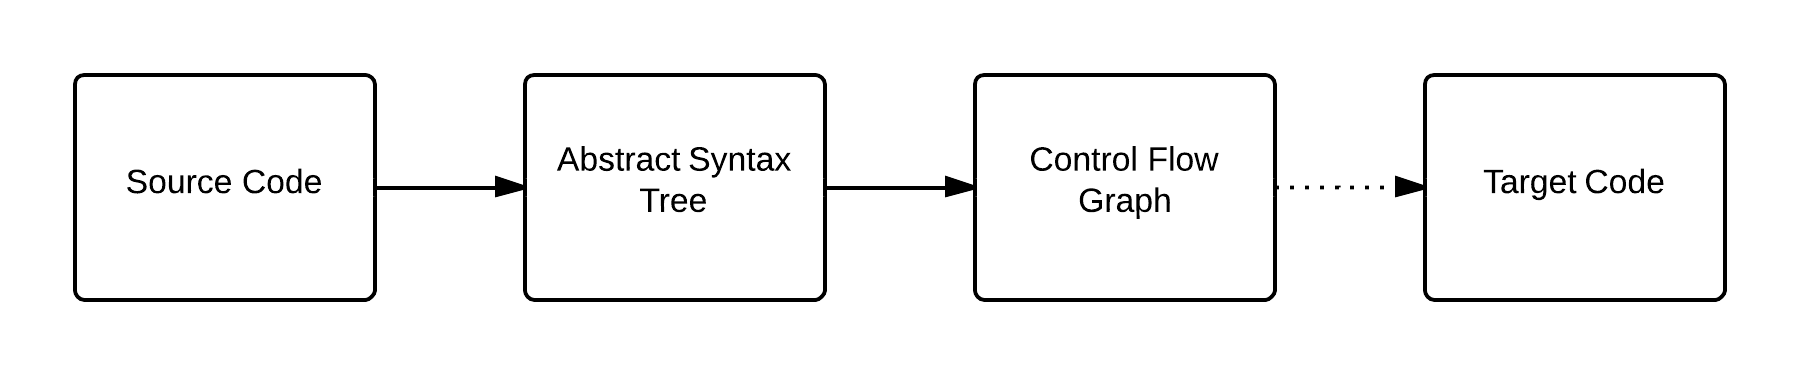
\includegraphics[width=0.8\linewidth]{figures/CompStructure}
\caption{Intermediate Representations}
\label{fig:Compiler}
\end{figure}

\section{Scala AST}
In this thesis, we do not create our own syntax trees representation but reuse the Scala Abstract Syntax Trees (AST) given freely by the Scala compiler's parser and type checker \cite{stocker2010scala}. This section gives necessary introduction to Scala AST to allow the reader to understand the transformation process from the source language to the target language. As described in the previous section, AST is one of the most important intermediate representations. The Scala compiler's parser and type checker provide the Scala AST as intermediate representation that we can directly work on. Additionally, the Scala compiler also provides a tool to traverse and transform an AST \cite{stocker2010scala}.

The Scala ASTs are the basis of abstract syntax which is used to represent programs. The Scala compiler uses ASTs as an intermediate representation before generating bytecode \cite{demarne2014scala}. In Scala reflection, Trees can be produced or used by the following APIs\footnote{http://lang.org/overviews/reflection/symbols-trees-types.html}:

\begin{itemize}
\item Scala annotations. This API uses the AST to represent their arguments and is exposed in \texttt{Annotation.scalaArgs}. 
\item \texttt{reify}. This special method takes an expression and returns an AST that represent this expression.
\item Compile time reflection with macros \cite{burmako2013scala} and runtime compilation with toolboxes use trees as their program representation medium. Macros expand trees at compile time allowing programmers to hack and manipulate AST within the compilation scope \cite{burmako2013scala}.
\end{itemize} 

\subsection{Scala Macros}
Compile time metaprogramming is the algorithmic construction of programs at compile-time. Scala macros is an experimental facility to allow user to perform compile-time metaprogramming \cite{burmako2012scala}. With this feature, compiler is enabled to recognize certain methods in Scala programs as metaprograms, or macros, which can be invoked at certain points. When invoked, macros expose a compiler context which includes the compiler's representation of the program being compiled along with an API that provides certain compiler functionality such as parsing and typechecking. Using these API, macros is able to affect compilation e.g. by changing the code being compiled \cite{burmako2013scala}.

$Def macros$, plain methods whose invocations are expanded during compilation, is the most basic form of compile-time metaprogramming and the one that we work with for this thesis. In the eye of the programmer, def macros appear to look like regular Scala methods with a special property-when a method in a Scala method satisfies this property, that macros definition is expanded by invoking a corresponding metaprogram, called $macro implementation$. The only fundamental difference with regular method is that macros are resolved at compile time  \cite{burmako2013scala}. An example of def macro implementation for \texttt{printf} function is depicted in Listing \ref{macros} below.
\begin{lstlisting}[language=scala,caption=Macros Printf Function \cite{burmako2013scala}, label = macros]
def printf(format: String, params: Any*): Unit = macro impl
def impl(c: Context)(format: c.Expr[String], params: c.Expr[Any]*): c.Expr[Unit] = ...
printf("Hello %s", "world")
\end{lstlisting}


\subsection{AST Classes}
This section introduces some of the concrete trees classes that are used in traversing the trees in our implementation. All concrete classes are case classes, thus their parameters are listed following the class name as follows \cite{stocker2010scala}. 
\begin{itemize}
\item \texttt{Block(stats: List[Tree], expr: Tree)}. A Block consists of a list of statements and returns the value of expr. As the name indicates, this class represents Block in the language grammar. 
\item \texttt{ValDef(mods: Modifiers, name: Name, tpt: Tree, rhs: Tree)}. Val- ue definitions are all definitions of vals, vars (identified by the MUTABLE flag) and parameters (identified by the param flag). In Scala, aside from value definitions, ValDef can also contain If statement. 
\item \texttt{LabelDef(name: Name, params: List[Ident], rhs: Tree)}. The Label- Def class is used to represent While and Do-While statement. The Scala language specification \cite{odersky2004scala} defines that the while loop statement \texttt{while(e1) e2} is typed and evaluated as if it is an application of \texttt{whileLoop(e1)(e2)} where the hypothetical function \texttt{whileLoop} is defined in Listing \ref{whileloop}. 
\begin{lstlisting}[language=scala,caption=WhileLoop Function, label = whileloop]
def whileLoop(cond: => Boolean)(body: => Unit): Unit = if (cond) { body ; whileLoop(cond)(body) } else {}
\label{def:program}
\end{lstlisting}
\item \texttt{Assign(lhs: Tree, rhs: Tree)}. Assign trees are used for non-initial assignments to variables. The lhs typically consists of an Ident(name) and is assigned the value of the rhs which normally contains an application (Apply) of a function. 
\item \texttt{If(cond: Tree, thenp: Tree, elsep: Tree)}. An If statement consists of three parts: the condition, the then part and the else part. If the else part is omitted, the literal () of type Unit is generated and the type of the conditional is set to an upper bound of Unit and the type of the then expression, usually Any. As the name indicates, this class represents the If statement in the language grammar. 
\end{itemize}

\subsection{Generating Scala AST}
Scala macros is used in this thesis to lift the root Block of a Scala program into a monatic comprehension of intermediate representation. We present a sample Scala program with iteration and an If statement inside the iteration (refer to Listing 1.2) and show the generated Scala AST of the program. 
\\
\begin{lstlisting}[language=scala, caption=Workflow with Conditional, label = workflow2]
val e1 = DataSource("/tmp/input1.txt", CsvInputFormat[(String, Int, Int)]())
          .filter(x => x._1 == "Joshua")
val e2 = DataSource("/tmp/input2.txt", CsvInputFormat[(String, Int, Int)]())
          .filter(x => x._1 == "Marten")
var e3: DataSet[(String, Int, Int)] = null
var i = 0

while(i < 0) {
if (e1.map(x => x._2).reduce((x, y) => Math.max(x, y)).fetch().head > 50)
        e3 = e1.map { x => (x._1, x._2 + 1000, x._3)}
    else
    	e3 = e2.map { x => (x._1, x._2 + 1500, x._3)}
i = i + 1
    }

val e4 = e3.write("/tmp/output.txt", CsvOutputFormat[(String, Int, Int)]())

e4
\end{lstlisting}

As shown in Scala AST in Figure 1.2, the program is represented by a Block which consists of list of statements and an expression which holds the final return value. Each of the variable definition is presented by a ValDef. The LabelDef in the AST represent the While statement in the program and consists of a name and a rhs of type If. The If statement consists of the three parts: condition, then part, and else part. In the while or LabelDef case, the else part which is of type Literal only contains an empty constant value. The then part is expanded to another list of statements and expression. Given that in the sample Scala program, there is a control flow inside the body of the loop, the statement then consists of another If statement. The then and else part of this If statement are of type Assign since in the program we assign a map function in the rhs to a variable name in the lhs. 

\begin{figure}[h!]
\centering
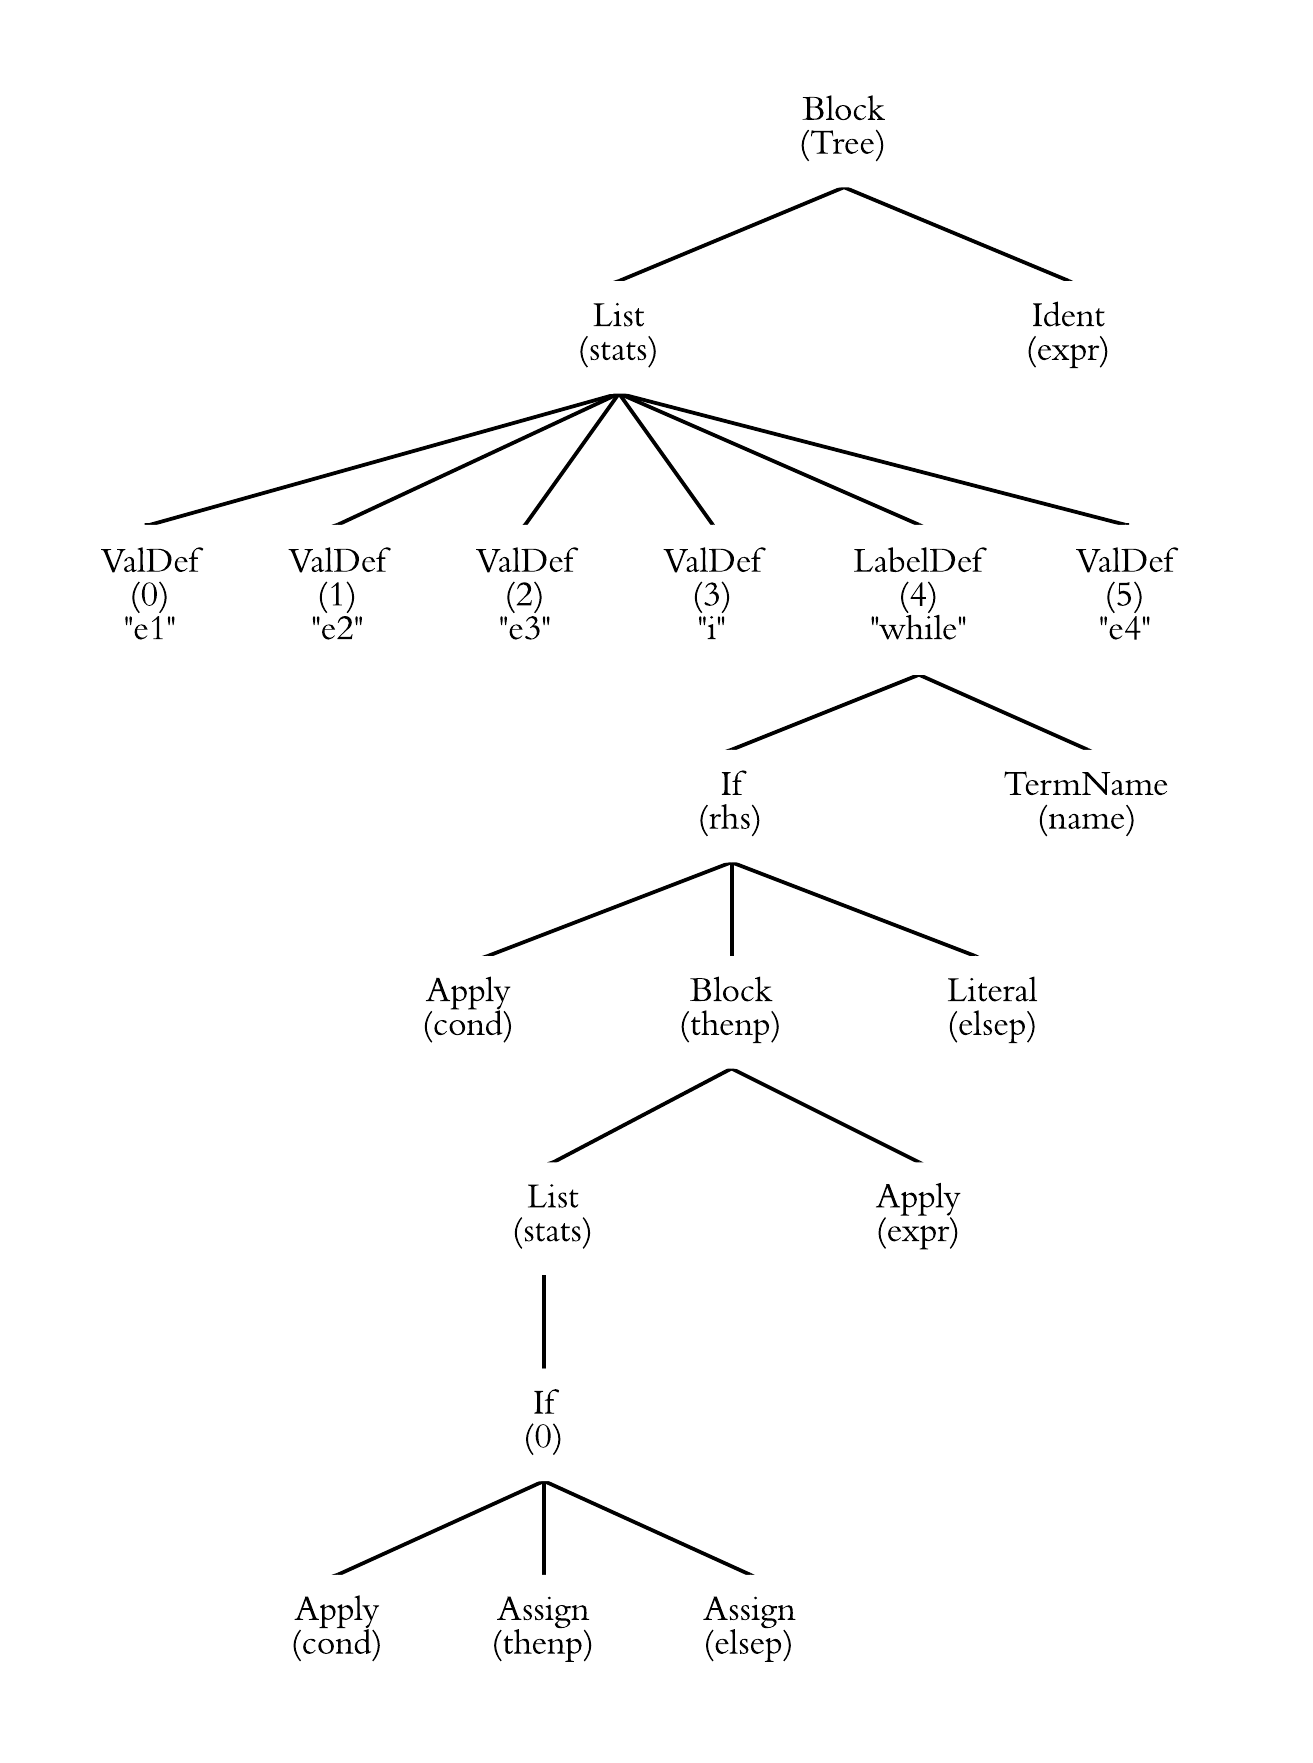
\includegraphics[width=0.8\linewidth]{figures/Tree}
\caption{Scala AST}
\label{fig:Tree}
\end{figure}

\section{Create CFG from AST Algorithm}
Creating CFG from AST is the first stage of the intermediate code and code generation process. This algorithm takes as an input a Scala AST and produces the output of a lower-level intermediate representation CFG $G=(V,E)$ with set $V$ of vertices and a set $E$ of directed edges. Each vertex $V$ is a sequence of one or multiple nodes $n$ in the AST. 

The idea is to traverse the tree from top to bottom starting from the $root$ and to visit each node $n$ of the children recursively. We check the type of each node $n$ and perform a set of actions accordingly. The procedure $createCFG(nCurr, G, vCurr, X)$ takes as input the following parameters. 
\begin{itemize}
\item $nCurr$ refers to the node that is currently being visited in the AST. In the beginning, $nCurr$ is initialized to root of the full AST of the program. Since we traverse the tree from top to bottom, the $nCurr$ becomes the root of the subtree of the initial root node. Depending on the type of the Tree, the $nCurr$ is either pushed to the current Vertex $vCurr$ or the subtree of the $nCurr$ is visited recursively. 

\item $G=(V,E)$ refers to the CFG produced by the procedure and is continuously being updated whenever recursion takes place. The CFG consists of a set of vertices and a set of directed edges. Each vertex of the resulted CFG is a sequence of statements or nodes in the AST. The vertices set $V$ of the graph has initial member of $vCurr$ whereas the edges set $E$ is initialized to an empty set.   

\item $vCurr$ refers to the vertex of the CFG that is currently being built. If the $nCurr$ or a subtree does not contain control flow or branches, the $nCurr$ will be pushed to the $vCurr$. Subsequently, if the subtree contains branches or control flow, new vertex will be added to the CFG as well as directed edges from the $vCurr$ to the new vertex. Furthermore, the new vertex will become the new $vCurr$ and the whole procedure of checking $nCurr$ for control flow is repeated. In the initialization, $vCurr$ is set to empty sequence since we just begin to traverse the tree. 

\item $X$ is a stack to store the variable which contains branches and needs to be updated with the return value of either the then part or the else part of the control flow. In the algorithm, this variable will be re-assigned to the return value and will be deleted from the stack allowing the stack empty at the end of the procedure.  

\end{itemize}

\begin{algorithm}[h]

\caption{Creating Control Flow Diagram from AST Part 1}\label{CFG}
\begin{algorithmic}[1]
\Initialize { $v_{curr}\gets [ ],V\gets \{v_{curr}\},E\gets \emptyset,X\gets [ ], n_{curr}\gets root$}
\Procedure{createCFG}{$n_{curr},G,v_{curr},X$}
\Switch {$n_{curr}$}
  \Case {$Block(stats,expr)$}
  	\For {each $s$ in $stats$}
  	\State $(G,v_{curr},X)\gets \Call{createCFG}{s,G, v_{curr},\emptyset}$
   	\EndFor  
    \State $(G,v_{curr},X)\gets \Call{createCFG}{expr,G, v_{curr},X}$
       	\State \textbf{return} $(G,v_{curr},X)$
      \EndCase
       
  \Case {$ValDef(name, rhs)$}
  		\If {$containsBranches(rhs)$}
  			\State $\Call{push}{ValDef(name,\emptyset),v_{curr}} $
  			\State $\Call{push}{name,X} $
  			\State $(G,v_{curr},X)\gets \Call{createCFG}{rhs,G, v_{curr},X} $
  		\Else
  			\State $\Call{push}{n_{curr}, v_{curr}} $
  		\EndIf
  	\State \textbf{return} $(G,v_{curr},X)$
  \EndCase

  \Case {$Assign(name,rhs)$}
    	\If {$containsBranches(rhs)$}
    		\State $\Call{push}{name,X} $
    		\State $(G,v_{curr},X)\gets \Call{createCFG}{rhs,G, v_{curr},X} $

    	\Else
    			\State $\Call{push}{n_{curr}, v_{curr}} $
    		\EndIf
    	\State \textbf{return} $(G,v_{curr},X)$
  \EndCase
  \Case {$While(cond,body)$}
  	\State $v_{condStart} \gets \Call{newV}$
  	\State $V \gets V \cup \{v_{condStart}\}; E \gets E \cup \{(v_{curr},v_{condStart})\}$ 
  	\State $(G,v_{condEnd},X)\gets \Call{createCFG}{cond,G,v_{condStart},\emptyset} $
  	\State $v_{bodyStart} \gets \Call{newV}{ }$
  	\State $V \gets V \cup \{v_{bodyStart}\}; E \gets E \cup \{(v_{condEnd},v_{bodyStart})\}$
  	\State $(G,v_{bodyEnd},X)\gets \Call{createCFG}{body,G, v_{bodyStart},\emptyset} $
  	\State $v_{curr} \gets \Call{newV}{ }$
  	\State $V \gets V \cup \{v_{curr}\}; E \gets E \cup \{(v_{condEnd},v_{curr}),(v_{bodyEnd},v_{condStart})\}$
  	\State \textbf{return} $(G,v_{curr},X)$
  \EndCase
 \algstore{bkbreak}
 \end{algorithmic}
 \end{algorithm}
 \begin{algorithm}
 \addtocounter{algorithm}{-1}
 \caption{Creating Control Flow Diagram from AST Part 2}\label{CFG2}
 \begin{algorithmic}[1]
 \algrestore{bkbreak}
  \Case {$DoWhile(cond,body)$}
      	\State $v_{bodyStart} \gets \Call{newV}{ }$
      	\State $V \gets V \cup \{v_{bodyStart}\}; E \gets E \cup \{(v_{curr},v_{bodyStart})\}$
  	\State $(G,v_{bodyEnd},X)\gets \Call{createCFG}{body,G, v_{body},\emptyset} $
  	\State $v_{condStart} \gets \Call{newV}{ }$
      	\State $V \gets V \cup \{v_{bodyEnd}, v_{condStart}\}; E \gets E \cup \{(v_{bodyEnd},v_{condStart})\}$ 
      	\State $(G,v_{condEnd},X)\gets \Call{createCFG}{cond,G,v_{cond},\emptyset} $
      	\State $v_{curr} \gets \Call{newV}{ }$
      	\State $V \gets V \cup \{v_{curr},v_{condEnd}\}$
      	\State $E \gets E \cup \{(v_{condEnd},v_{curr}),(v_{condEnd},v_{bodyStart})\}$
      	\State \textbf{return} $(G,v_{curr},X)$
    \EndCase
  \Case {$If(cond,thenp,elsep)$}
  	\State $(G,v_{cond},X)\gets \Call{createCFG}{cond,G, v_{cond},\emptyset}$
  	\State $v_{thenp} \gets \Call{newV}{ }$
  	\State $V \gets V \cup \{ v_{thenp}; E \gets E \cup \{(v_{curr},v_{thenp})\}$
  	\State $(G,v_{thenp},X)\gets \Call{createCFG}{thenp,G, v_{thenp},X} $
  	
  	\State $v_{elsep} \gets \Call{newV}{ }$
  	\State $V \gets V \cup \{v_{elsep}\};E \gets E \cup \{(v_{curr},v_{elsep})$
  	\State $(G,v_{elsep},X)\gets \Call{createCFG}{elsep,G, v_{elsep},X} $
  	
  	\State $v_{curr} \gets \Call{newV}{ }$
  	\State $V \gets V \cup \{v_{curr}\};E \gets E \cup \{(v_{thenp},v_{curr}),(v_{elsep},v_{curr})\}$
 	  	
  	\State \textbf{return} $(G,v_{curr},X)$
    	
  \EndCase

  \Case { $\_$}
  	\If {$X \neq \emptyset$}
	\State $name \gets X.head$
  	\State $\Call{push}{Assign(name,n_{curr}),v_{curr}} $ 
  	\Else
  	\State $\Call{push}{n_{curr},v_{curr}} $ 
  	\EndIf 
  	\State \textbf{return} $(G,v_{curr},X)$
  	
  \EndCase
 
\EndSwitch
\EndProcedure
\Procedure{containsBranches}{$n_{curr}$}
\Switch {$n_{curr}$}
  \Case {$Block(_,expr)$}
  \State $\Call{containsBranches}{expr}$
  \EndCase
  \Case {$If(\_)$}
  	\State \textbf{return} $true$
  \EndCase
  \Case {$\_$}
    \State \textbf{return} $false$
    \EndCase
\EndSwitch
\EndProcedure
\end{algorithmic}
\end{algorithm}

Using Scala pattern matching, we are able to traverse the tree and match the current node of the tree $nCurr$ to a Scala AST type. Based on its type, the following procedure will be taken. 

\begin{itemize}

\item $Block(stats, expr)$.
A Block typically consists of a list of statements and an expression. For every statement inside the Block, the procedure is called recursively and the Graph $G=(V,E)$, current vertex $vCurr$, and stack of variable $X$ are subsequently updated. After each statement is visited, the procedure is also called recursively for the single expression.  

\item $ValDef(name,rhs)$
As mentioned in the Scala AST introduction section, ValDef refers to definition of a variable both immutable (val) and mutable (var). In this case, we check whether the ValDef contains branches or control flow. If there is a control flow inside the ValDef, the same ValDef with a mutable identifier is pushed to the current vertex $vCurr$ and the name of the variable of type TermName is stored in the stack variable $X$. The name of the variable needs to be stored because it must be assigned later on with the value in the Then part or the Else part of the control flow. The rhs then becomes the current node $nCurr$ and the procedure is called recursively.  Sample program that will encounter this case is provided in the Listing 1.3 below. In this case, the variable $e3$ is stored in $X$ and later will be assigned to the function "e1.map {..}" or function "e2.map {..}".
\begin{lstlisting}[language=scala,caption=ValDef with Branches, label = valdef]
val e3 = if (e1.map(x => x._2).reduce((x, y) => Math.max(x, y)).fetch().head > 50)
	e1.map { x => (x._1, x._2 + 1000, x._3)}
else
	e2.map { x => (x._1, x._2 + 1500, x._3)}
\end{lstlisting}

If the ValDef does not contain branches, then the current node $nCurr$ is simply pushed to the current vertex $vCurr$. 

\item $Assign(name,rhs)$
The procedure for the case Assign is similar with ValDef. We check whether the tree or node contains branches. If it does, the name of the variable is stored in the stack variable $X$ to be assigned later on with the value in the Then part or the Else part of the control flow. The procedure is then called recursively with the rhs as the new current node $nCurr$. Similar to ValDef, if the Tree does not contain branches, the current node $nCurr$ is simply pushed to the current vertex $vCurr$.

\item $While(cond,body)$
As depicted in Figure 2-3, for While loop, a new vertex $vCondStart$ is created to store the condition of the iteration. A directed edge is defined from the current vertex $vCurr$ to the new vertex $vCondStart$. A new vertex $vBodyStart$ is also created to store the statements in the $body$ of the iteration. Both the $cond$ and $body$ may or may not contain branches. Hence, recursive call both for $cond$ and $body$ take place which results in the new vertex $vCondEnd$ and $vBodyEnd$ respectively. A directed edge is defined from the end of the $body$ which is the vertex $vBodyEnd$ to the beginning of the $cond$ which is the vertex $vCondStart$. At the end, a new vertex is created as the new current vertex $vCurr$ and a directed edge is defined from the vertex $vBodyEnd$ to the new current vertex $vCurr$. 

\item $DoWhile(cond,body)$
The procedure for DoWhile case is similar with While case with the differences in the order the vertices are created as well as the directed edges connecting the vertices. The $vBodyStart$ is created first and is connected to the $vCurr$. The vertex result of the recursive call to the body of the iteration, vertex $vBodyEnd$ is connected to the new vertex $vCondStart$ which stores the condition of the iteration. The end of the condition $vCondEnd$ is connected to the start of the $body$ $vBodyStart$. Similar to the While loop, at the end, a new vertex is created as the new current vertex $vCurr$ and a directed edge is defined from the vertex $vCondEnd$ to the new current vertex $vCurr$. 

\item $If(cond,thenp,elsep)$
At first, we create a new vertex $vCond$ to store the condition of the If statement. A directed edge is connected from the current vertex $vCurr$ to the $vCond$. A recursive call is performed to the procedure since the $cond$ may or may not contain branches. We then create two new vertices $vThenp$ and $vElsep$ to represent the Then part and the Else part of the If statement consecutively. A directed edge is defined from $vCond$ to both new vertices $vThenp$ and $vElsep$ to represent all possible flows. Recursive call is performed both for the Then part $thenp$ and Else part $elsep$ since they may or may not contain branches. At the end, a new vertex is created as the new current vertex $vCurr$ and a directed edge is defined both from the vertex $vThenp$ and vertex $vElsep$ to the new current vertex $vCurr$. 

\item $Default Case)$
We first check whether the stack of variable $X$ contains any member. If yes, then we have get the last member inserted to $X$ which is a name, and assign the current node $nCurr$ to the name. This assignment is then pushed to the current vertex $vCurr$. If the stack variable $X$ does not contain any member, which means no assignment is needed, the current node $nCurr$ is simply pushed to the current vertex $vCurr$. 
\end{itemize}

We perform this algorithm with the input of the Scala AST of the program in Listing 2-1. The CFG result is shown in Figure 1.4. 

\begin{figure}[h!]
\centering
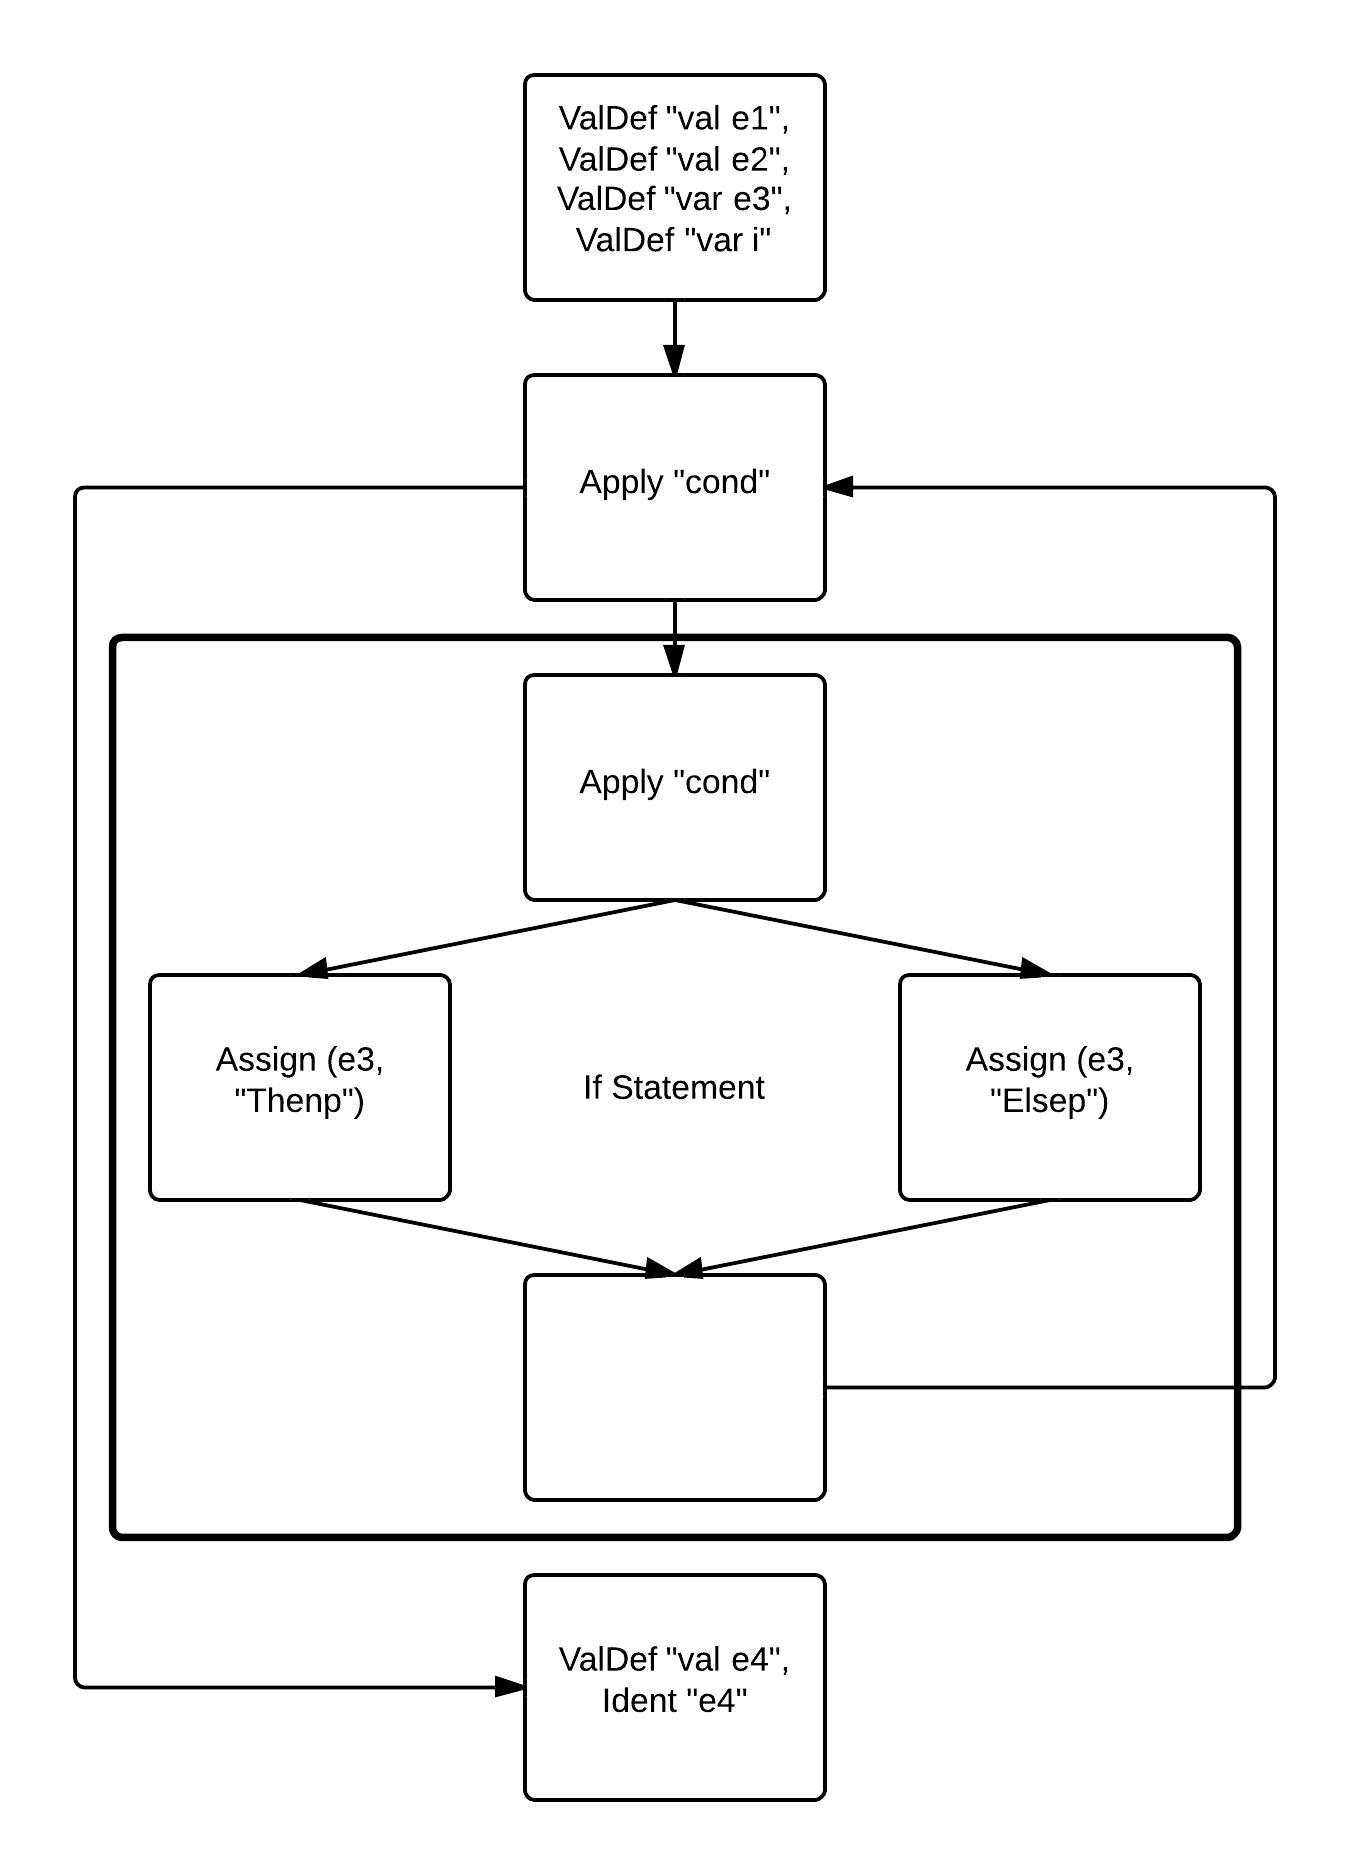
\includegraphics[width=0.7\linewidth]{figures/FinalGraph}
\caption{CFG of Scala AST of sample Program}
\label{fig:FinalGraph}
\end{figure}



